\documentclass[12pt]{article}
\usepackage{graphicx}
\usepackage{caption}
\usepackage{placeins}
\usepackage{amsmath}
\begin{document}

\section*{Part 1 -  Magnetic Field around a straight wire}
\subsection*{procedure and goal}

We set up a power source, ammeter, and straight wire in series. We had a probe which could measure the magnetic field at any point in space.We completed two different experiments. In the first experiment we measured the magnetic field around the straight wire with a fixed distance but varying current. In the second experiment we measured the magnetic field around the straight wire with a fixed current but varying distance.  

\subsection*{results}
	
	\begin{table}[hp]
	\caption{With a fixed distance}
	\centering
	\begin{tabular}{|r|r|}
	\hline 
	I(amperes) & B(Gauss) \\
	\hline 
	0.00 & .041 \\
	1.00 & .168 \\
	1.23 & .217 \\
	1.51 & .254 \\
	2.03 & .320 \\
	2.23 & .336 \\
	2.60 & .369 \\
	\hline
	\end{tabular}
	\end{table}

	\begin{table}[hp] 
	\caption{With fixed current}
	\centering
	\begin{tabular}{|r|r|r|}
	\hline 
	N(turns) & B(Gauss) & 1/B(Gauss) \\
	\hline 
	0 & .318 & 3.144 \\
	2 & .296 & 3.37 \\
	4 & .283 & 3.53 \\
	6 & .244 & 4.09\\
	8 & .223 & 4.48 \\
	10 & .211 & 4.73 \\
	12 & .188  & 5.31\\
	\hline
	\end{tabular}
	\end{table}

	\begin{figure}[hp]
	 \centering
	 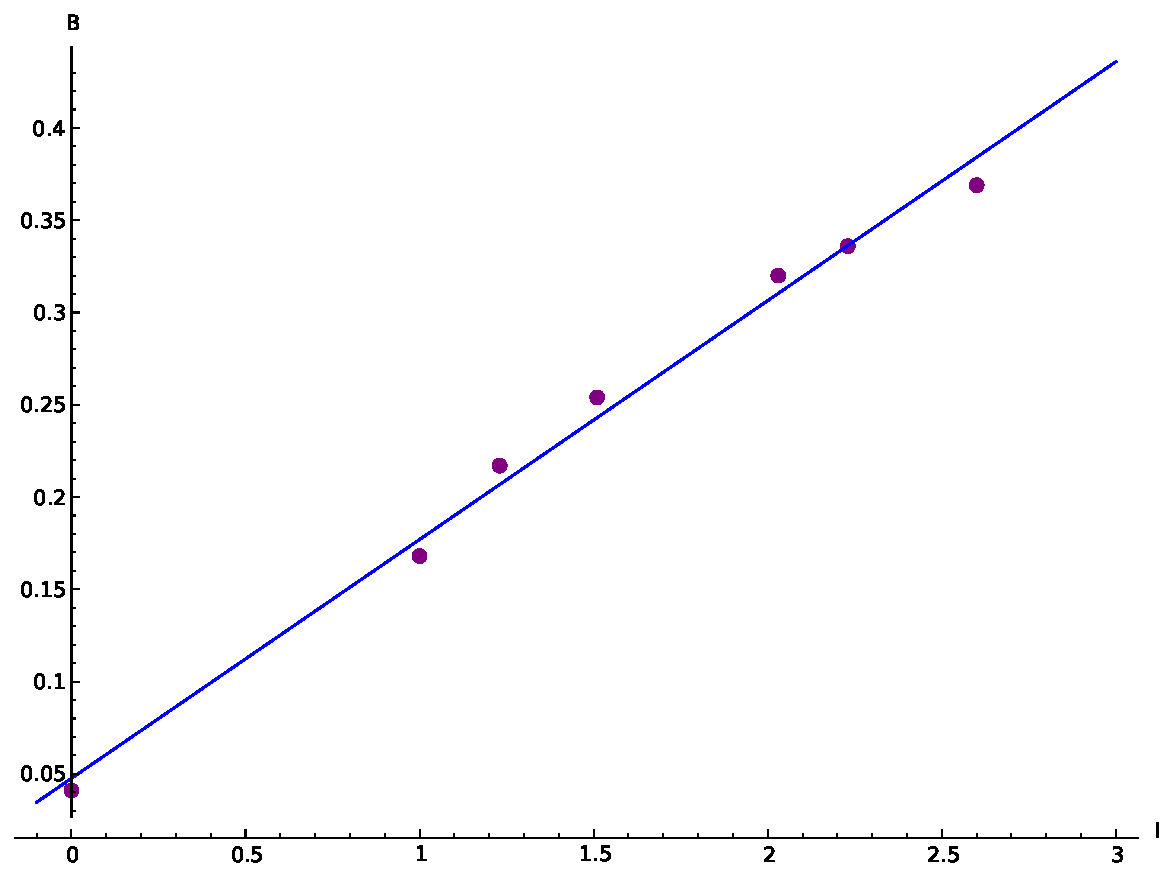
\includegraphics[scale = .85]{plot1}
	 \caption*{table 1 data: $I$ vs $B$. Best fit line is $B = .129I + .047$}
	\end{figure} 

	\begin{figure}[hp]
	 \centering
	 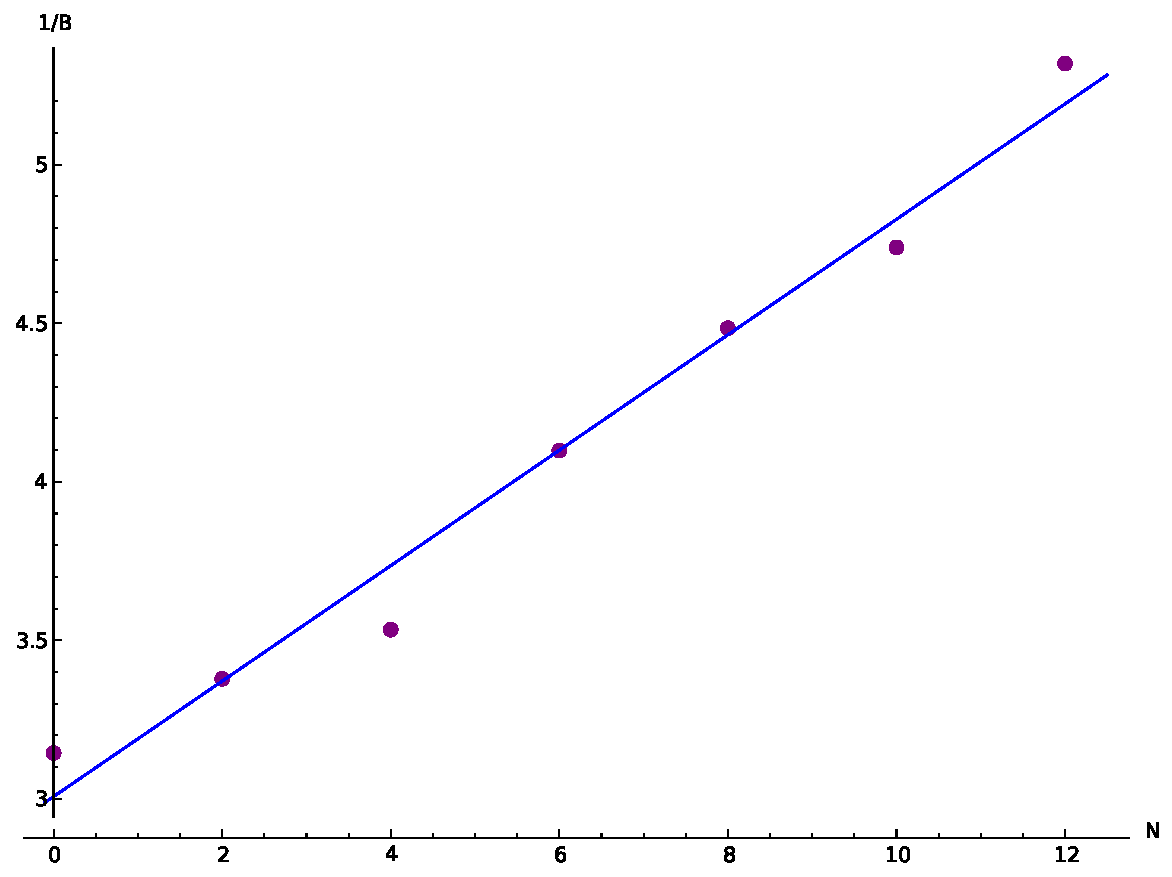
\includegraphics[scale = .85]{plot2}
	 \caption*{table 2 data: $N$ vs $\frac{1}{B}$. Best fit Line is $ \frac{1}{B} = .18N + 3 $}
	\end{figure}
	\FloatBarrier

\subsection*{analysis}



\section*{part 2 - Magnetic Field around Magnet}

\subsection*{procedure and goal}

\subsection*{results} 
	\begin{table}[h]
	\caption{}
	\centering
	\begin{tabular}{|r|r|r|}
	\hline 
	D(cm) & B(Gauss) & 1/B(Gauss) \\
	\hline 
	2.5 & 1.41 & .709 \\
	3.5 & 1.21 & .826 \\
	4.5 & .914 & 1.09 \\
	5.5 & .274 & 3.64 \\
	6.5 & .07 & 14.28 \\
	\hline
	\end{tabular}
	\end{table}

	\begin{figure}[hp]
	 \centering
	 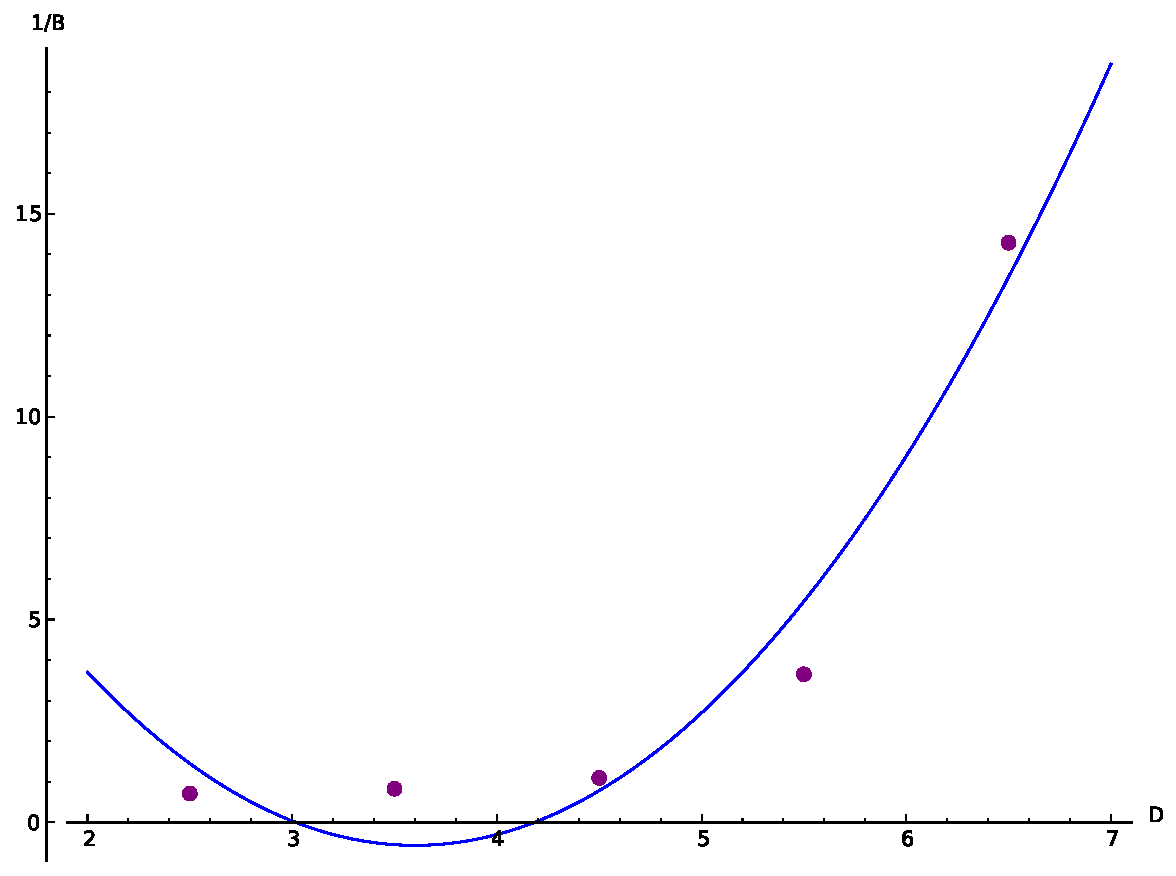
\includegraphics[scale = .85]{plot3}
	 \caption*{table 3 data: $D$ vs $\frac{1}{B}$. Best fit quadratic was $ \frac{1}{B} = 1.66D^2  - 11.99D + 21.03 $}
	\end{figure} 

	\begin{figure}[hp]
	 \centering
	 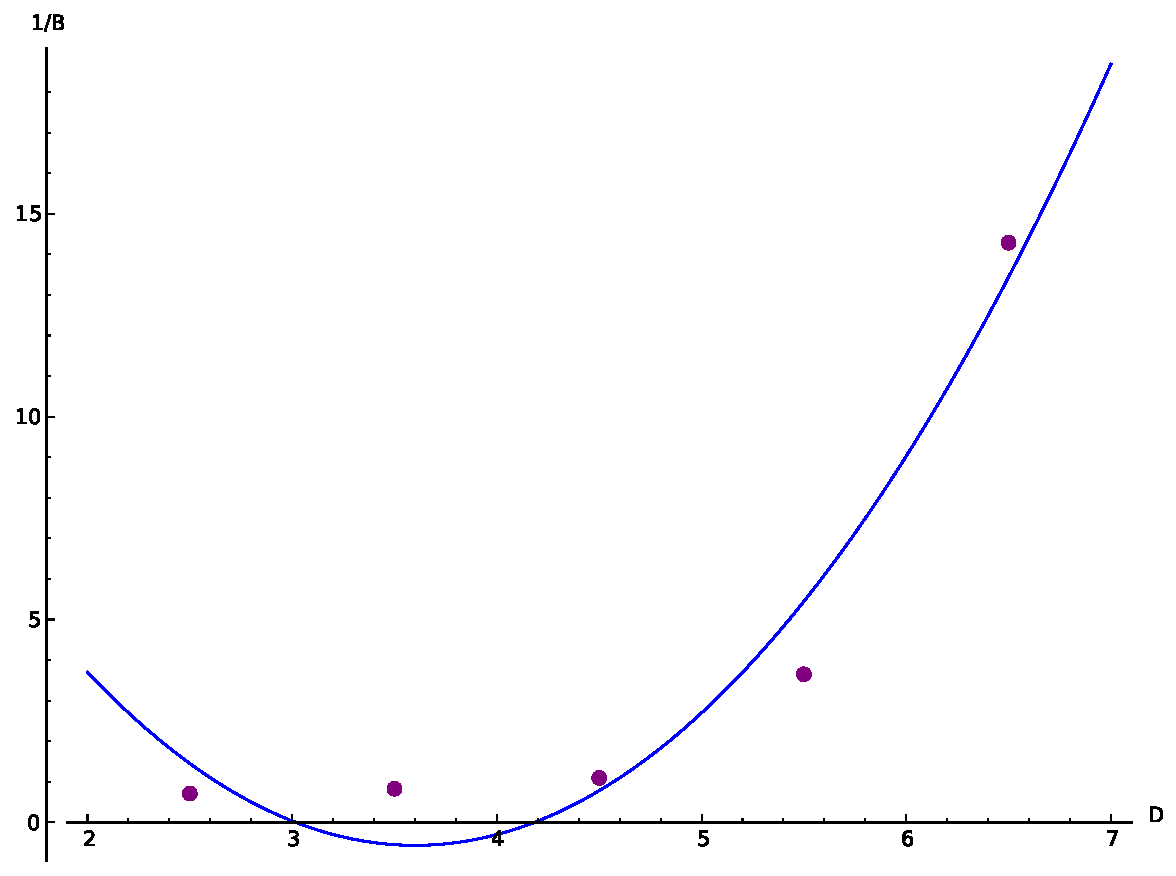
\includegraphics[scale = .85]{plot3}
	 \caption*{table 3 data: $D$ vs $\frac{1}{B}$. Best fit cubic was $ \frac{1}{B} = .066D^3  - 7.25D^2 + 25.9D - 29.07 $}
	\end{figure} 
	\FloatBarrier

\subsection*{analysis}




\end{document}
